\chapter{Design}

\section{Class Diagram}

\begin{figure}[htbp]
\centering
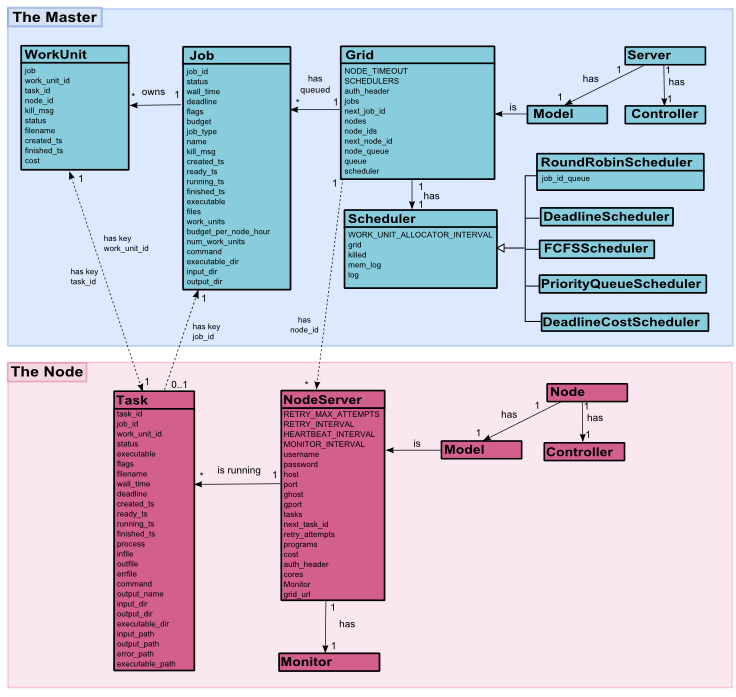
\includegraphics[keepaspectratio,width=\textwidth,height=0.75\textheight]{./figs/class.png}
\caption{New Job Creation}
\end{figure}

\section{Sequence Diagrams}

\begin{figure}[htbp]
\centering
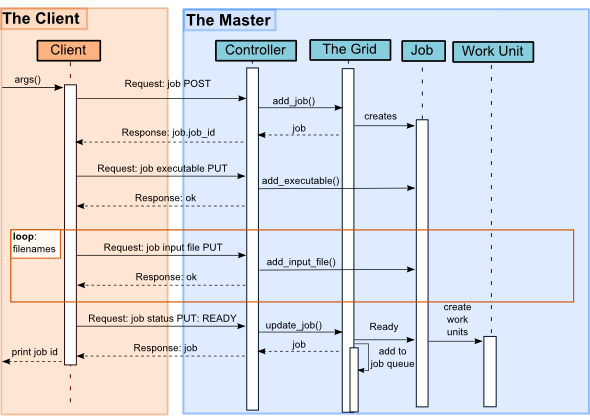
\includegraphics[keepaspectratio,width=\textwidth,height=0.75\textheight]{./figs/jobcreate.png}
\caption{New Job Creation}
\end{figure}


\begin{figure}[htbp]
\centering
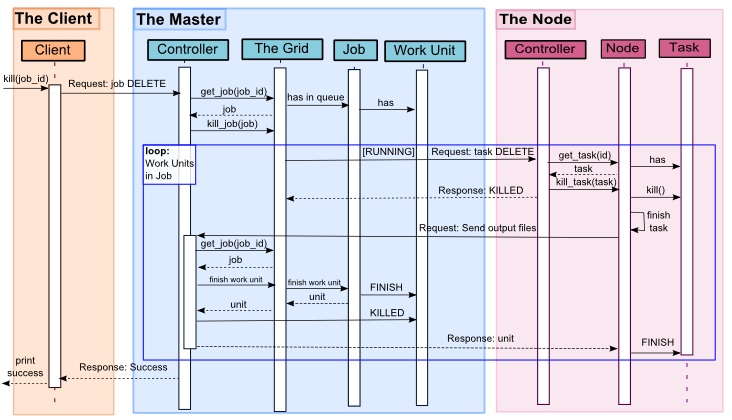
\includegraphics[keepaspectratio,width=\textwidth,height=0.75\textheight]{./figs/jobkill.png}
\caption{Kill a Job}
\end{figure}


\begin{figure}[htbp]
\centering
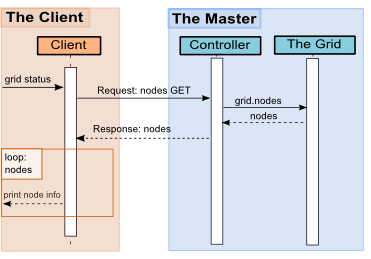
\includegraphics[keepaspectratio,width=\textwidth,height=0.75\textheight]{./figs/gridstatus.png}
\caption{Get the status of The Grid}
\end{figure}


\begin{figure}[htbp]
\centering
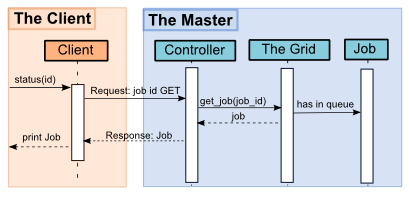
\includegraphics[keepaspectratio,width=\textwidth,height=0.75\textheight]{./figs/jobget.png}
\caption{Get the status of a Job}
\end{figure}


\begin{figure}[htbp]
\centering
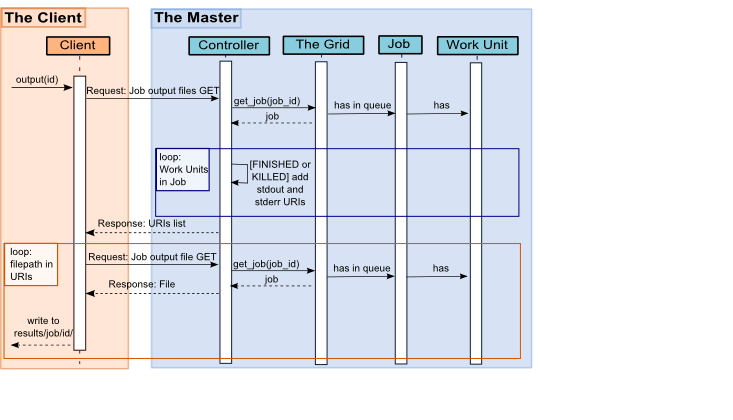
\includegraphics[keepaspectratio,width=\textwidth,height=0.75\textheight]{./figs/getoutput.png}
\caption{Get the output of a finished Job}
\end{figure}


\begin{figure}[htbp]
\centering
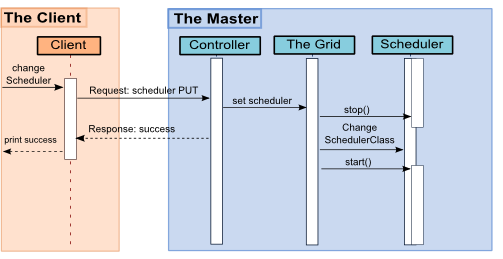
\includegraphics[keepaspectratio,width=\textwidth,height=0.75\textheight]{./figs/scheduler.png}
\caption{Change the scheduler dynamically}
\end{figure}


\begin{figure}[htbp]
\centering
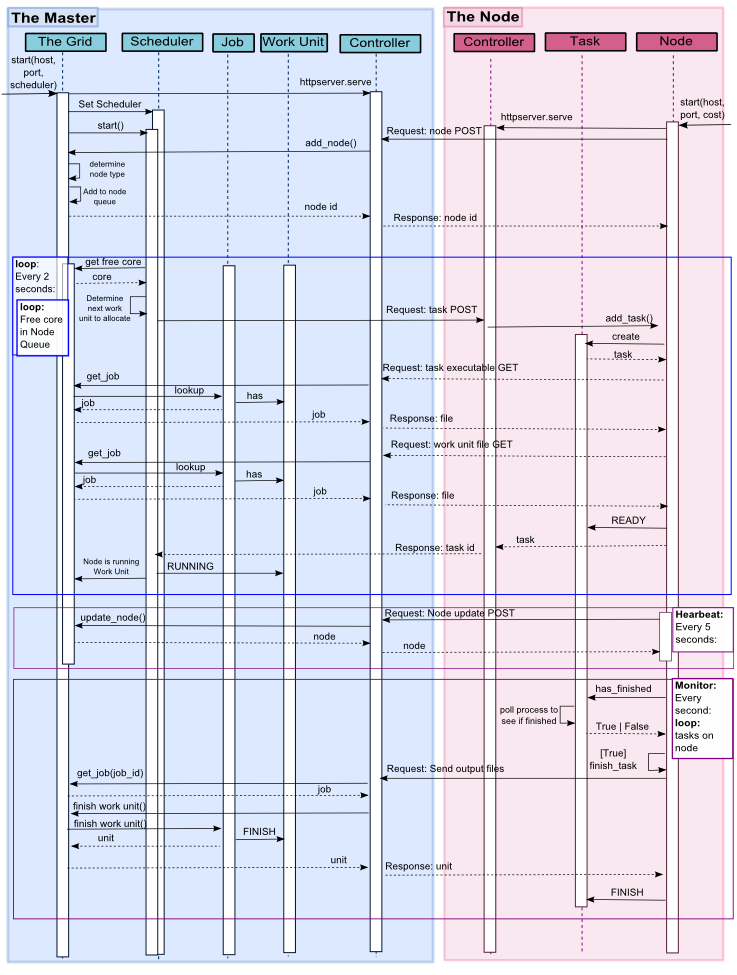
\includegraphics[keepaspectratio,width=\textwidth,height=0.75\textheight]{./figs/servernode.png}
\caption{Interaction between The Master and The Nodes in The Grid}
\end{figure}

